\documentclass[aspectratio=169,10pt]{beamer}

\usepackage[utf8]{inputenc}
\usepackage[T1]{fontenc}
\usepackage{lmodern}
\usepackage{amsmath,amssymb}
\usepackage{booktabs}
\usepackage{graphicx}
\usepackage{array}
\usepackage{tikz}
\usepackage{xcolor}

\graphicspath{{paper/final/assets/}{./paper/final/assets/}}

\definecolor{ink}{HTML}{17212B}
\definecolor{muted}{HTML}{5D6773}
\definecolor{soft}{HTML}{EEF3F6}
\definecolor{line}{HTML}{D6E0E6}
\definecolor{daBlue}{HTML}{2467A8}
\definecolor{daTeal}{HTML}{12807A}
\definecolor{daGreen}{HTML}{2B7A3D}
\definecolor{daGold}{HTML}{A77A13}
\definecolor{daCoral}{HTML}{C8553D}

\setbeamertemplate{navigation symbols}{}
\setbeamertemplate{headline}{}
\setbeamertemplate{itemize item}{\raisebox{0.15ex}{\scriptsize$\blacktriangleright$}}
\setbeamertemplate{itemize subitem}{\raisebox{0.15ex}{\tiny$\bullet$}}
\setbeamertemplate{footline}{%
  \hfill{\scriptsize\color{muted}\insertframenumber/\inserttotalframenumber}\hspace{1.2em}\vspace{0.7em}%
}

\setbeamercolor{normal text}{fg=ink,bg=white}
\setbeamercolor{frametitle}{fg=ink,bg=white}
\setbeamercolor{framesubtitle}{fg=muted,bg=white}
\setbeamerfont{frametitle}{series=\bfseries,size=\Large}
\setbeamerfont{framesubtitle}{size=\small}

\newcommand{\sectionlabel}[1]{%
  {\color{muted}\scriptsize\MakeUppercase{#1}}\vspace{0.35em}
}

\newcommand{\keybox}[3]{%
  \begin{tikzpicture}
    \node[
      fill=#1!9,
      draw=#1!35,
      rounded corners=3pt,
      inner xsep=7pt,
      inner ysep=6pt,
      text width=#2,
      align=left
    ] {\small #3};
  \end{tikzpicture}
}

\newcommand{\metricrow}[3]{#1 & #2 & #3\\}

\title{Scene-Assimilated Video World Models}
\subtitle{Retrieval-Guided Data Assimilation for Image-to-Video Generation}
\author{Daniel Yu}
\institute{Data Assimilation + Machine Learning Final Project}
\date{\today}

\begin{document}

\begin{frame}[plain]
  \vspace{1.0em}
  {\color{muted}\small Data Assimilation + Machine Learning Final Project}

  \vspace{1.1em}
  {\LARGE\bfseries Scene-Assimilated\\Video World Models}

  \vspace{0.45em}
  {\large\color{muted}Retrieval-guided data assimilation for image-to-video generation}

  \vspace{1.0em}
  \begin{columns}[T,totalwidth=\textwidth]
    \begin{column}{0.54\textwidth}
      \keybox{daBlue}{0.92\linewidth}{
        \textbf{Core idea.}
        A retrieved real video is not just extra prompt context.
        It is treated as a sparse scene observation that corrects an open-loop video forecast.
      }

      \vspace{0.8em}
      {\footnotesize
      \begin{tabular}{@{}>{\color{ink}}p{0.22\linewidth}p{0.70\linewidth}@{}}
        \textcolor{daBlue}{Forecast} & image-to-video rollout from anchor image and prompt \\
        \textcolor{daTeal}{Observation} & retrieved real-video trajectory \\
        \textcolor{daGreen}{Analysis} & denoising representation after observation fusion
      \end{tabular}
      }
    \end{column}
    \begin{column}{0.40\textwidth}
      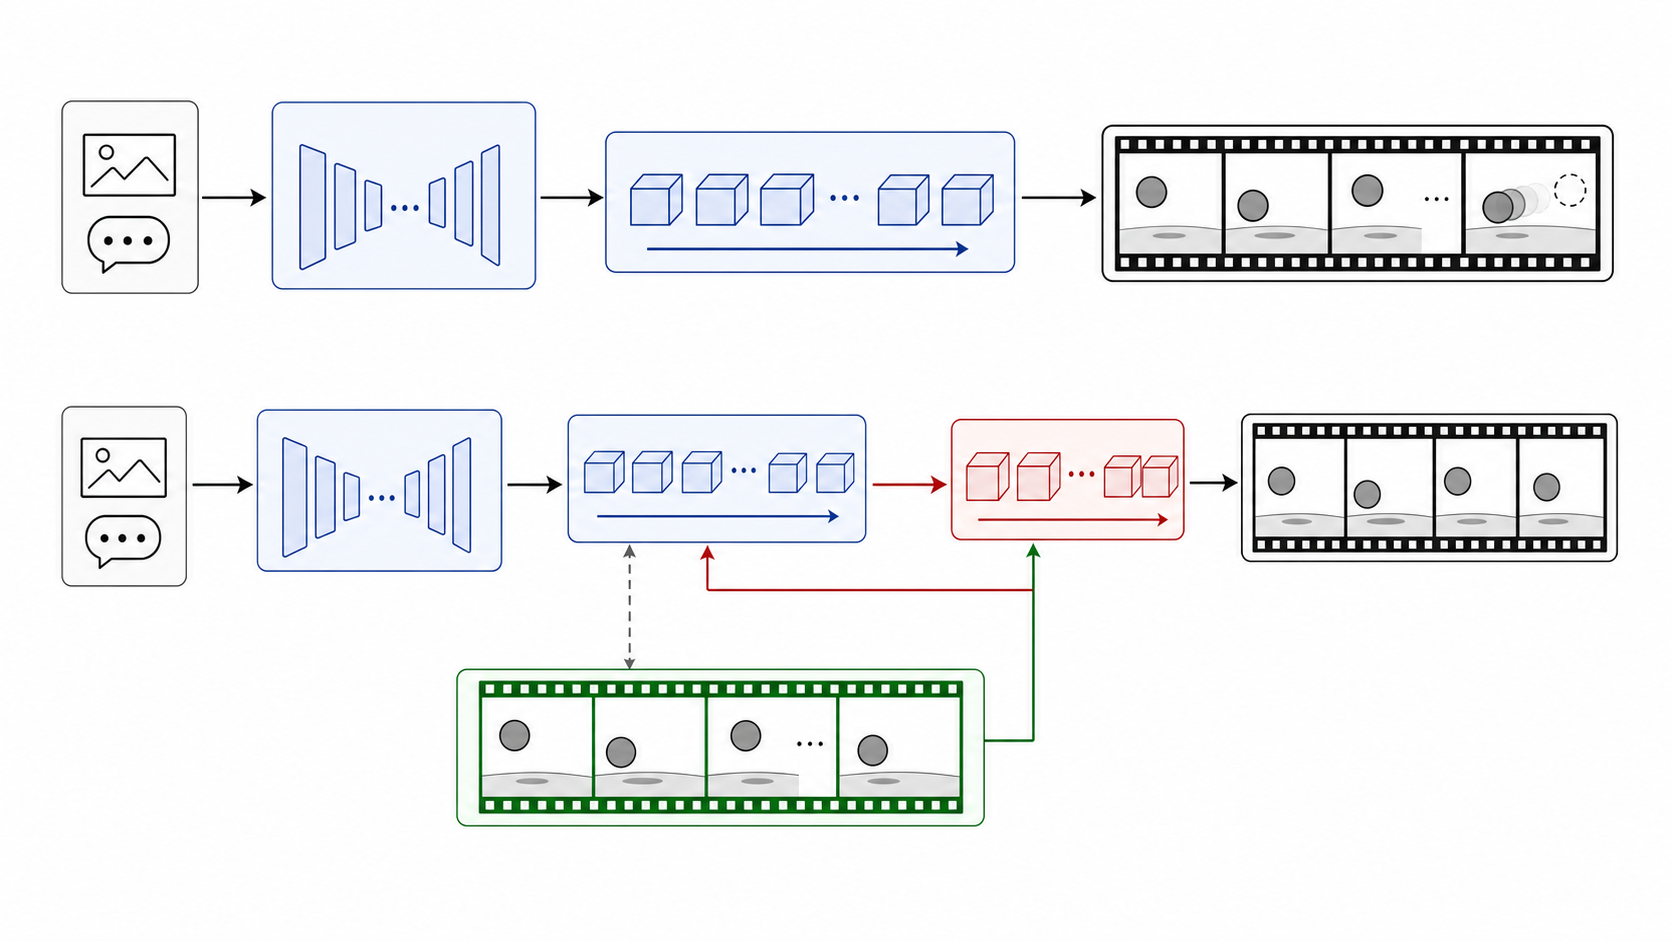
\includegraphics[width=\linewidth]{intro_concept_imagegen.png}
    \end{column}
  \end{columns}
\end{frame}

\begin{frame}[t]{Motivation: Open-Loop Video World Models}
\sectionlabel{problem}

\begin{columns}[T,totalwidth=\textwidth]
  \begin{column}{0.50\textwidth}
    
\includegraphics[width=\linewidth,height=0.72\textheight,keepaspectratio]{observation_analysis_paradigm_manual.png}
  \end{column}
  \begin{column}{0.46\textwidth}
    {\large\bfseries Image-to-video generation behaves like a world model.}

    \vspace{0.35em}
    \begin{itemize}
      \setlength\itemsep{0.42em}
      \item Input: one anchor image and a short prompt.
      \item Output: a plausible future trajectory of the scene.
      \item Failure point: the model must infer dynamics that text and one image do not specify.
    \end{itemize}

    \vspace{0.35em}
    \keybox{daCoral}{0.92\linewidth}{
      Prompts such as ``a surfer riding a wave'' omit contact timing, acceleration, camera motion, water deformation, and scene-level parallax.
    }
  \end{column}
\end{columns}
\end{frame}

\begin{frame}[t]{Thesis: Retrieval as Sparse Scene Observation}
\sectionlabel{paradigm}

\begin{columns}[T,totalwidth=\textwidth]
  \begin{column}{0.48\textwidth}
    {\large\bfseries Reframing retrieval}

    \vspace{0.45em}
    \begin{itemize}
      \setlength\itemsep{0.42em}
      \item Retrieval is often used as semantic context or a reference to copy.
      \item Here, the retrieved clip is a partial empirical trajectory from a related real scene.
      \item The clip should correct under-specified dynamics without overwriting the anchor image.
    \end{itemize}
  \end{column}
  \begin{column}{0.48\textwidth}
    {\large\bfseries Data assimilation view}

    \vspace{0.45em}
    \[
      p(x_t\mid y_{1:t})
      \propto
      p(y_t\mid x_t)\,p(x_t\mid y_{1:t-1})
    \]

    \vspace{0.35em}
    \[
      x^{a}
      =
      x^{f}
      +
      \frac{P^{f}}{P^{f}+R}(y-x^{f})
    \]

    \vspace{0.1em}
    {\small
    The equations are not claimed as exact for video DiTs; they define the role of each component:
    forecast, observation, innovation, and analysis.
    }
  \end{column}
\end{columns}

\vspace{0.8em}
\begin{center}
  \keybox{daGreen}{0.82\linewidth}{
    Scene-assimilated generation asks where real observations enter the latent transition state of the generator.
  }
\end{center}
\end{frame}

\begin{frame}[t]{Controlled Evidence: Moving MNIST Latent ETKF}
\sectionlabel{sanity check}

\begin{columns}[T,totalwidth=\textwidth]
  \begin{column}{0.48\textwidth}
    {\large\bfseries Why this experiment?}

    \vspace{0.45em}
    \begin{itemize}
      \setlength\itemsep{0.55em}
      \item The final video generator is too expensive for explicit ensemble DA.
      \item Moving MNIST gives a controlled setting where latent state correction can be measured.
      \item If observation is genuinely assimilated, the information gap between forecast and analysis should shrink.
    \end{itemize}

    \vspace{0.55em}
    \[
      D_{\mathrm{KL}}(p_a\|p_f)
      =
      \int p_a(z)\log\frac{p_a(z)}{p_f(z)}\,dz
    \]
    \[
      I(Z;Y)=H(Z)-H(Z\mid Y)
    \]
  \end{column}
  \begin{column}{0.48\textwidth}
    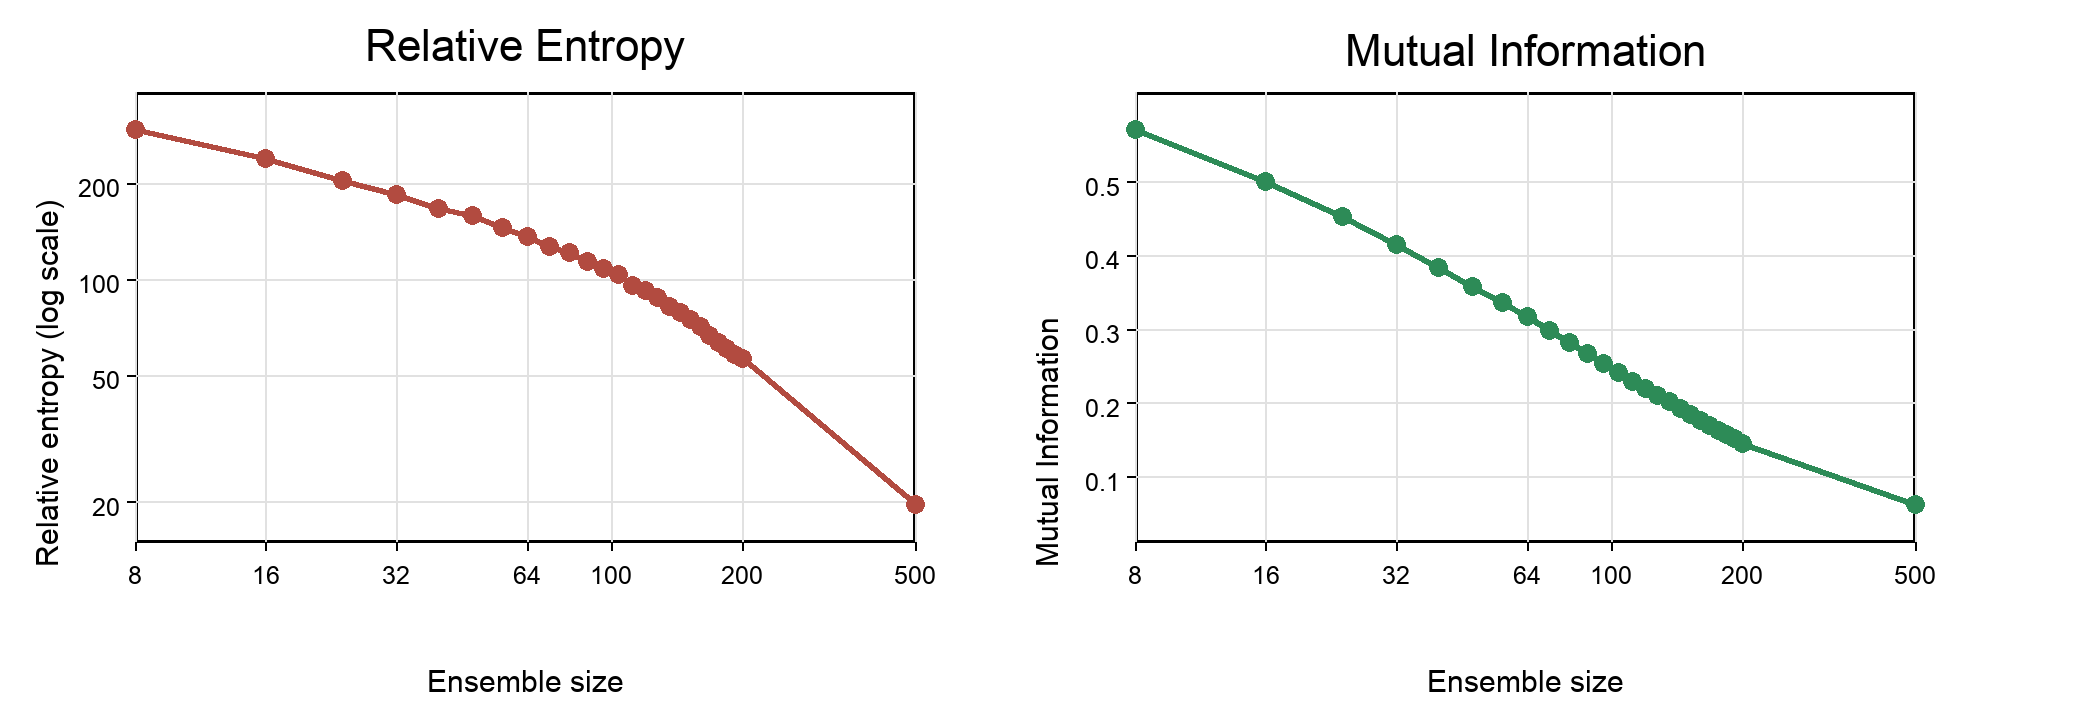
\includegraphics[width=\linewidth]{etkf_information_metrics.png}

    \vspace{0.2em}
    {\small
    \begin{tabular}{lcc}
      \toprule
      ETKF ensemble & $D_{\mathrm{KL}}\downarrow$ & residual $I(Z;Y)\downarrow$\\
      \midrule
      \metricrow{8 members}{295.4926}{0.5709}
      \metricrow{100 members}{105.9172}{0.2477}
      \metricrow{500 members}{19.6006}{0.0622}
      \bottomrule
    \end{tabular}
    }
  \end{column}
\end{columns}
\end{frame}

\begin{frame}[t]{Method Overview}
\sectionlabel{retrieval-guided data assimilation}

\begin{columns}[T,totalwidth=\textwidth]
  \begin{column}{0.58\textwidth}
    
\includegraphics[width=\linewidth]{method_analysis_embedded_manual.png}
  \end{column}
  \begin{column}{0.38\textwidth}
    {\large\bfseries Three components}

    \vspace{0.45em}
    \begin{itemize}
      \setlength\itemsep{0.55em}
      \item \textbf{Retrieval memory:} OpenVid-style real videos indexed by LanguageBind.
      \item \textbf{Two streams:} forecast tokens from the generator and observation tokens from retrieved video.
      \item \textbf{Analysis update:} in-context DiT attention fuses both streams before noise prediction.
    \end{itemize}
  \end{column}
\end{columns}
\end{frame}

\begin{frame}[t]{Retrieval Memory as Observation Source}
\sectionlabel{observation selection}

\begin{columns}[T,totalwidth=\textwidth]
  \begin{column}{0.47\textwidth}
    {\large\bfseries Memory bank}

    \vspace{0.5em}
    \[
      \mathcal{R}=\{(r_i,c_i)\}_{i=1}^{N}
    \]
    \[
      q = Q_{\mathrm{LB}}(I,p)
    \]
    \[
      (r^{\star},c^{\star})
      =
      \arg\max_{(r_i,c_i)\in\mathcal{R}} s(q,r_i)
    \]

    \vspace{0.4em}
    {\small
    The query combines anchor image $I$ and prompt $p$.
    The retrieved clip $r^\star$ is a nearby real-world trajectory, not the target video.
    }
  \end{column}
  \begin{column}{0.49\textwidth}
    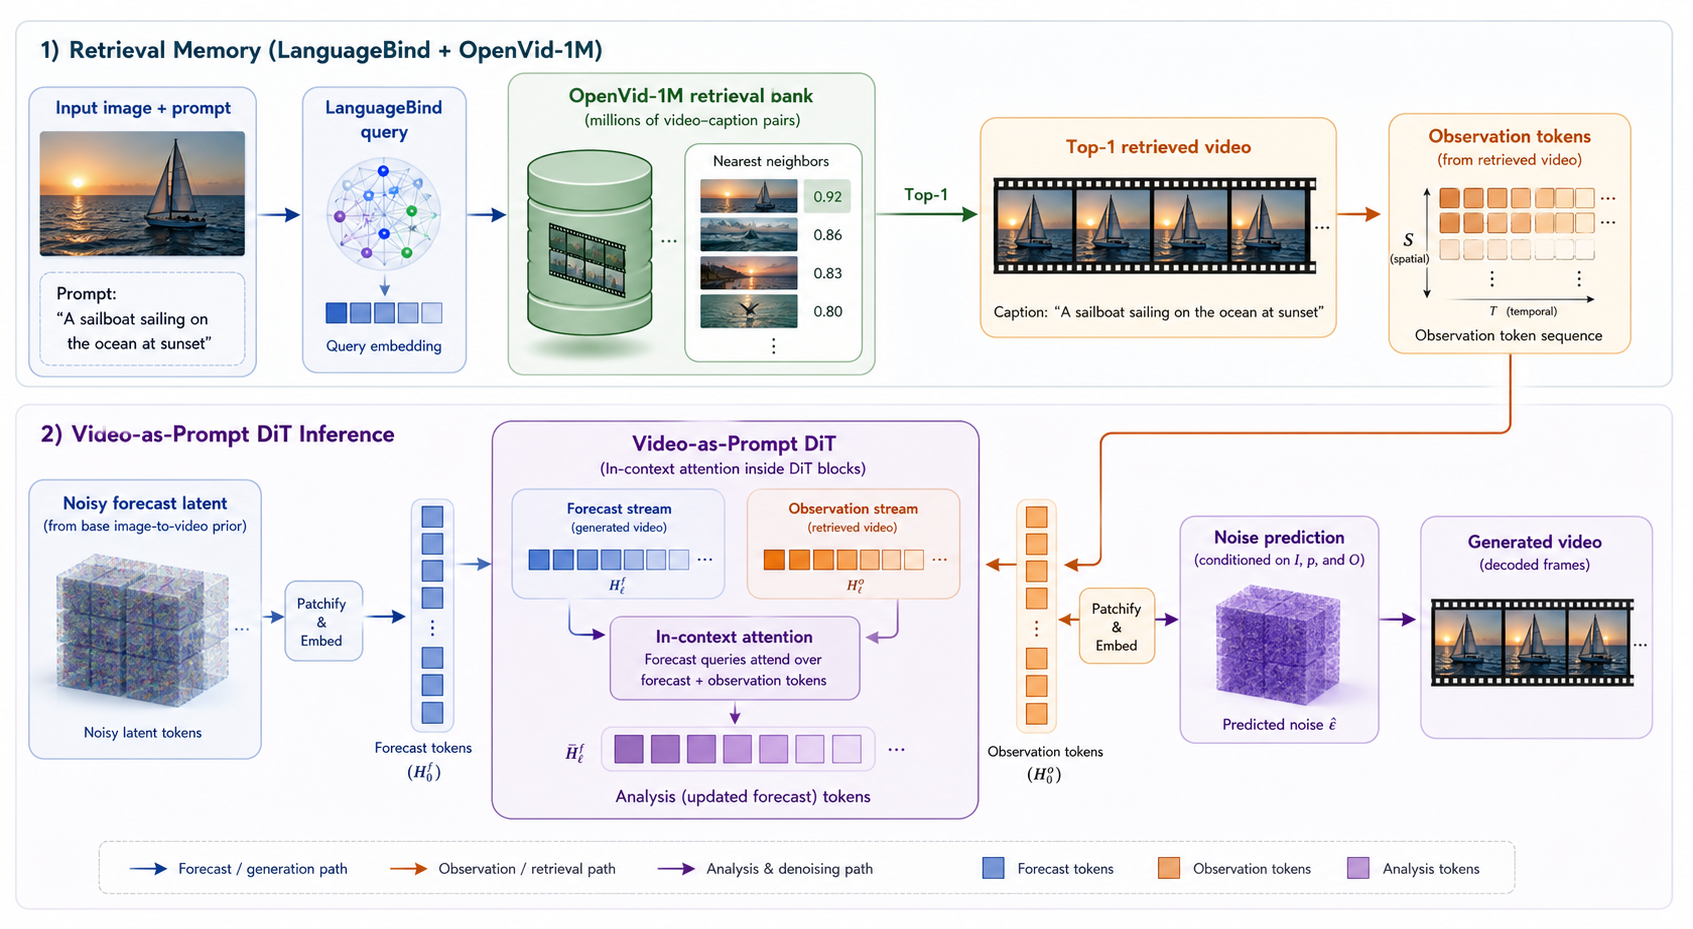
\includegraphics[width=\linewidth]{retrieval_vap_architecture_imagegen.png}
  \end{column}
\end{columns}
\end{frame}

\begin{frame}[t]{Analysis Inside the DiT}
\sectionlabel{learned state update}

\begin{columns}[T,totalwidth=\textwidth]
  \begin{column}{0.50\textwidth}
    {\large\bfseries Forecast and observation streams}

    \vspace{0.4em}
    \[
      H_0^{f}=P_{\mathrm{patch}}(z_t^{f},I,p)
    \]
    \[
      O = E_{\mathrm{vid}}(r^{\star},c^{\star}),
      \qquad
      H_0^{o}=P_{\mathrm{obs}}(O)
    \]

    \vspace{0.45em}
    \keybox{daBlue}{0.90\linewidth}{
      The forecast stream preserves the generator's own rollout.
      The observation stream carries real-video dynamics.
    }
  \end{column}
  \begin{column}{0.46\textwidth}
    {\large\bfseries Attention as analysis operator}

    \vspace{0.25em}
    \[
      \bar{H}_{\ell}^{f}
      =
      \operatorname{Attn}
      \left(
      Q_{\ell}^{f},
      \begin{bmatrix}K_{\ell}^{f}\\K_{\ell}^{o}\end{bmatrix},
      \begin{bmatrix}V_{\ell}^{f}\\V_{\ell}^{o}\end{bmatrix}
      \right)
    \]

    \[
      z_t^{a}=\mathcal{A}_{\theta}(z_t^{f},O,I,p)
    \]
    \[
      \hat{\epsilon}=\epsilon_{\theta}(z_t^{f},t,I,p,O)
    \]
  \end{column}
\end{columns}
\end{frame}

\begin{frame}[t]{Fine-Tuning Objective}
\sectionlabel{training}

\begin{columns}[T,totalwidth=\textwidth]
  \begin{column}{0.48\textwidth}
    {\large\bfseries What is trained?}

    \vspace{0.45em}
    \begin{itemize}
      \setlength\itemsep{0.55em}
      \item Keep the base image-to-video DiT, VAE, and text encoder frozen.
      \item Fine-tune the retrieval-guided in-context pathway.
      \item Use the target clip for denoising supervision and a non-identical retrieved clip as observation.
    \end{itemize}
  \end{column}
  \begin{column}{0.48\textwidth}
    {\large\bfseries Conditional diffusion loss}

    \vspace{0.45em}
    \[
      \mathcal{L}_{\mathrm{ft}}
      =
      \mathbb{E}_{x,I,p,r^\star,c^\star,t,\epsilon}
      \left[
      \left\|\epsilon-
      \epsilon_{\theta}(z_t,t,I,p,r^\star,c^\star)
      \right\|_2^2
      \right]
    \]

    \vspace{0.4em}
    \keybox{daTeal}{0.90\linewidth}{
      This keeps the architecture modular: base generator as forecast model, retrieval bank as world memory, in-context pathway as analysis update.
    }
  \end{column}
\end{columns}
\end{frame}

\begin{frame}[t]{Wan2.1 Pilot Setup}
\sectionlabel{qualitative evaluation}

\begin{columns}[T,totalwidth=\textwidth]
  \begin{column}{0.45\textwidth}
    {\large\bfseries Comparison}

    \vspace{0.35em}
    \begin{itemize}
      \setlength\itemsep{0.42em}
      \item Baseline: Wan2.1-14B image-to-video from image and prompt.
      \item Ours: same input plus one retrieved real-video observation through the VAP-style pathway.
      \item Six short-prompt cases: basketball, swing, dog, horse, surfing, and running.
    \end{itemize}

    \vspace{0.35em}
    \keybox{daGold}{0.92\linewidth}{
      A mechanism check under prompt under-specification, not a completed benchmark.
    }
  \end{column}
  \begin{column}{0.51\textwidth}
    
\includegraphics[width=\linewidth,height=0.68\textheight,keepaspectratio]{qualitative_six_case_late_panel.png}
  \end{column}
\end{columns}

\end{frame}

\begin{frame}[t]{Qualitative Results: Motion Becomes More Active}
\sectionlabel{results}

\begin{columns}[T,totalwidth=\textwidth]
  \begin{column}{0.56\textwidth}
    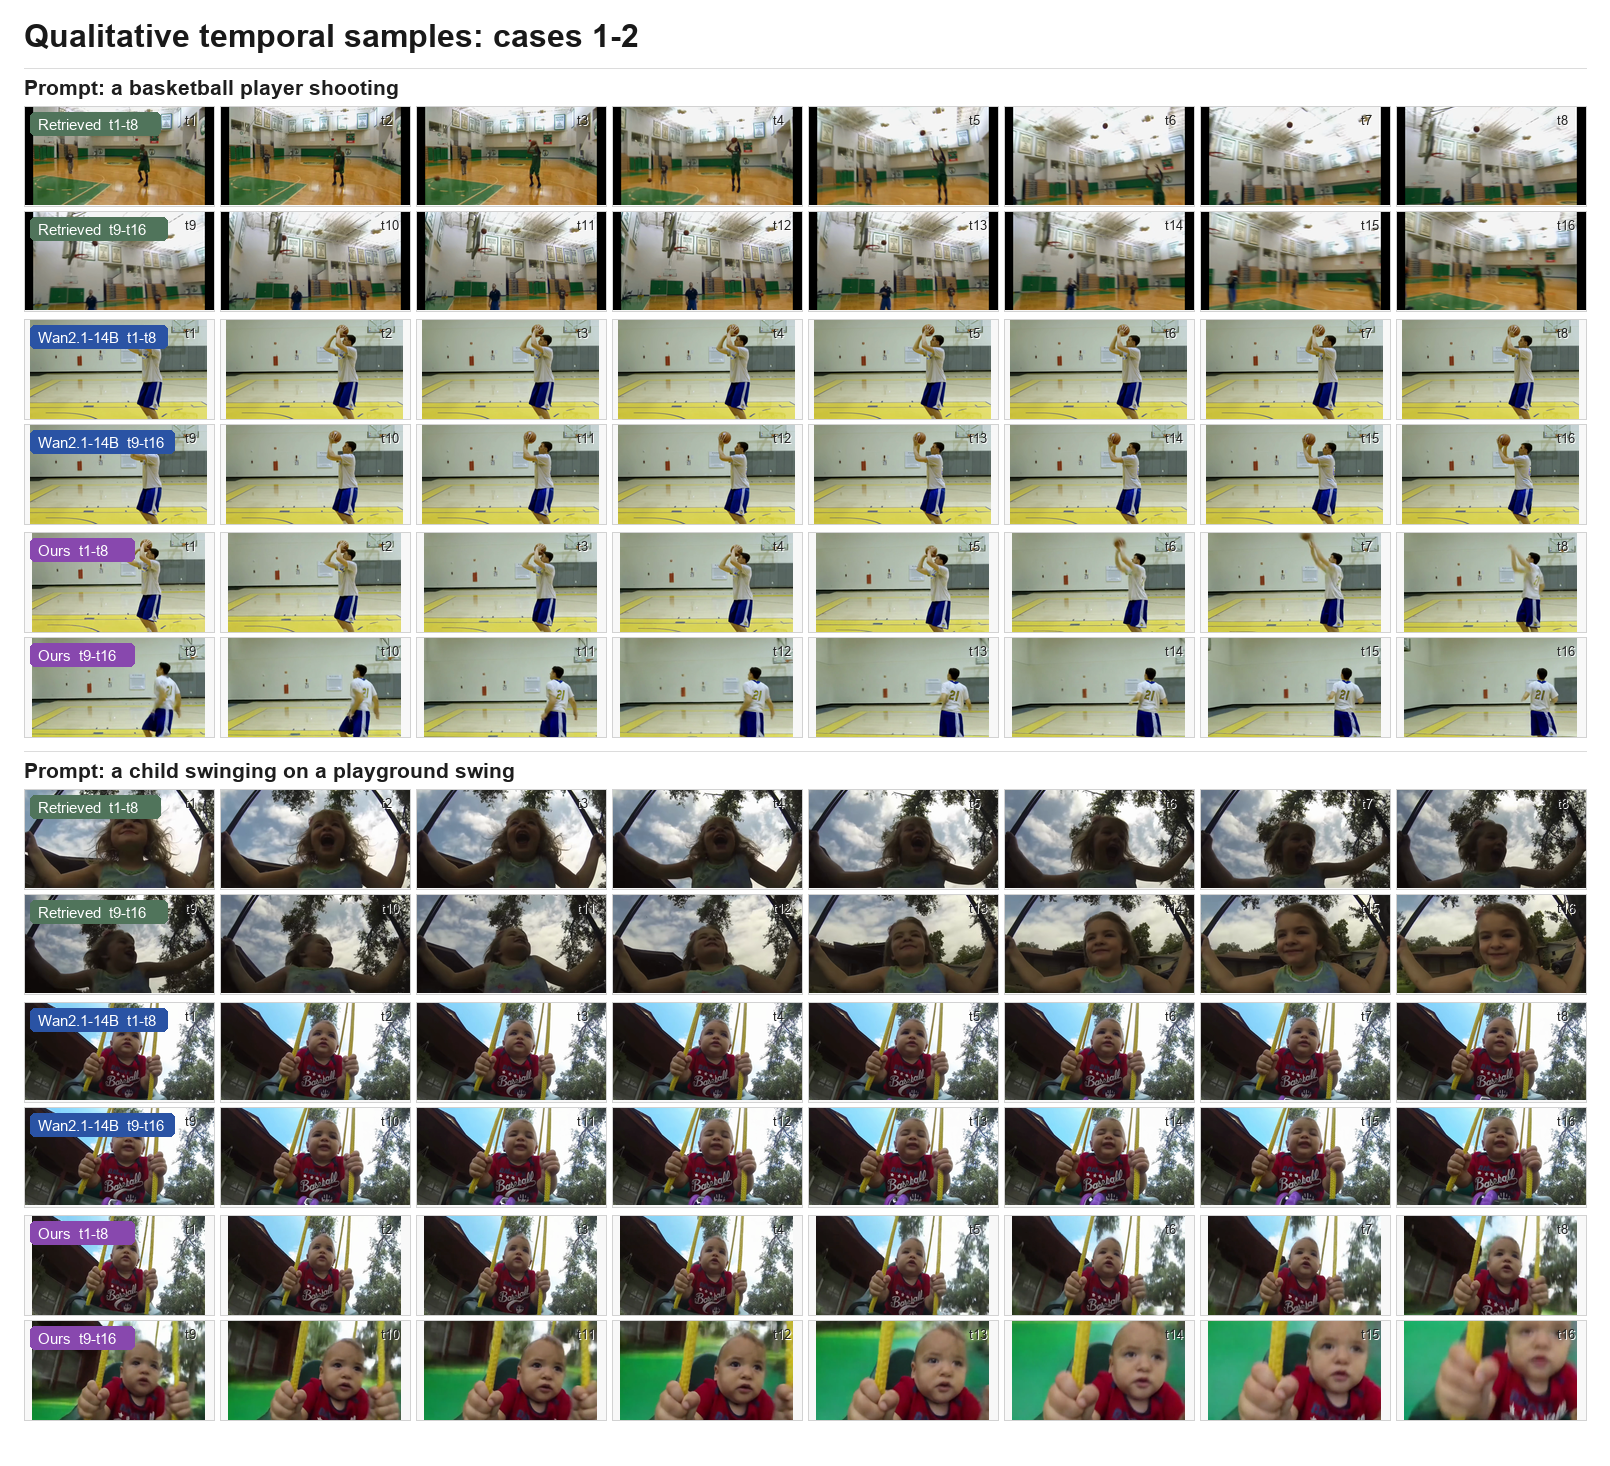
\includegraphics[width=\linewidth,height=0.74\textheight,keepaspectratio]{qualitative_temporal_panel_1.png}
  \end{column}
  \begin{column}{0.40\textwidth}
    {\large\bfseries Observed pattern}

    \vspace{0.45em}
    \begin{itemize}
      \setlength\itemsep{0.55em}
      \item Basketball: clearer shooting trajectory and follow-through.
      \item Swing: stronger depth and camera motion.
      \item Dog, horse, surfing, running: more body, scene, and background dynamics.
    \end{itemize}

    \vspace{0.45em}
    \keybox{daGreen}{0.92\linewidth}{
      Retrieval helps most when the prompt leaves physical evolution ambiguous and the retrieved clip is spatially compatible.
    }
  \end{column}
\end{columns}
\end{frame}

\begin{frame}[t]{Failure Modes Are Part of the Claim}
\sectionlabel{limits}

\begin{columns}[T,totalwidth=\textwidth]
  \begin{column}{0.55\textwidth}
    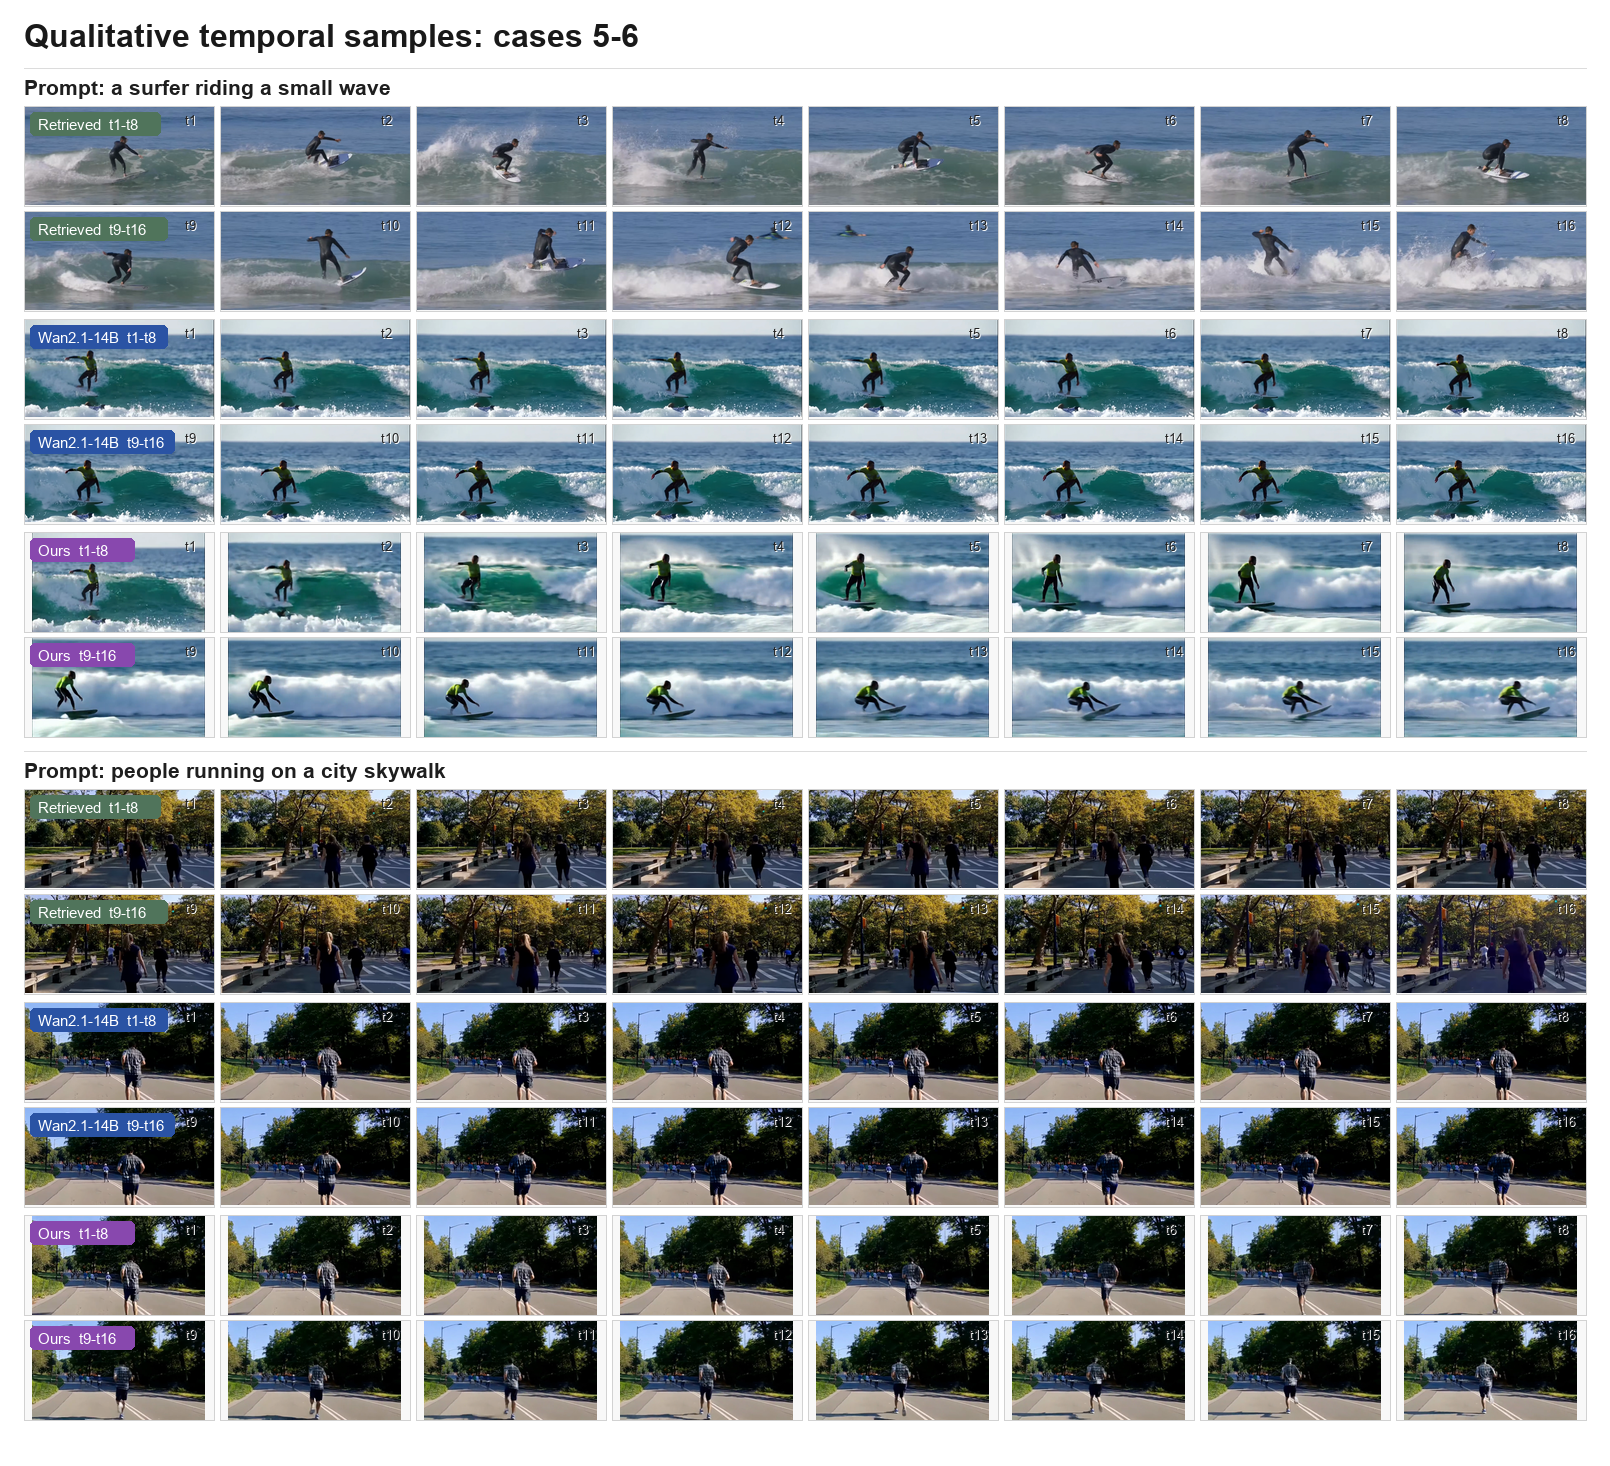
\includegraphics[width=\linewidth,height=0.74\textheight,keepaspectratio]{qualitative_temporal_panel_3.png}
  \end{column}
  \begin{column}{0.41\textwidth}
    {\large\bfseries Observation can be too strong}

    \vspace{0.45em}
    \begin{itemize}
      \setlength\itemsep{0.55em}
      \item Mismatched viewpoint can introduce framing drift.
      \item Mismatched subject scale or identity can soften details.
      \item More motion is not automatically a better world model.
    \end{itemize}

    \vspace{0.45em}
    \keybox{daCoral}{0.92\linewidth}{
      The real tradeoff is physical consistency versus spatial anchoring.
      A robust analysis operator must learn how much to trust the retrieved observation.
    }
  \end{column}
\end{columns}
\end{frame}

\begin{frame}[t]{Benchmark Implication}
\sectionlabel{what should be measured}

\begin{columns}[T,totalwidth=\textwidth]
  \begin{column}{0.31\textwidth}
    \keybox{daBlue}{0.94\linewidth}{
      \textbf{Motion}

      Dynamic degree, action accuracy, temporal smoothness, optical-flow plausibility.
    }
  \end{column}
  \begin{column}{0.31\textwidth}
    \keybox{daTeal}{0.94\linewidth}{
      \textbf{Spatial anchoring}

      Subject consistency, background consistency, identity preservation, framing stability.
    }
  \end{column}
  \begin{column}{0.31\textwidth}
    \keybox{daGreen}{0.94\linewidth}{
      \textbf{World-model behavior}

      Physical consistency, causal event evolution, retrieval-alignment stratification.
    }
  \end{column}
\end{columns}

\vspace{0.65em}
{\large\bfseries Expected result is conditional, not uniform.}

\vspace{0.35em}
\begin{itemize}
  \setlength\itemsep{0.35em}
  \item Aligned observations should improve motion and physical consistency.
  \item Mismatched observations may reduce identity, sharpness, or background stability.
  \item Reporting only aggregate quality can hide whether the model actually assimilates useful evidence.
\end{itemize}
\end{frame}

\begin{frame}[t]{Takeaways}
\sectionlabel{conclusion}

\begin{columns}[T,totalwidth=\textwidth]
  \begin{column}{0.48\textwidth}
    {\large\bfseries Contributions}

    \vspace{0.3em}
    \begin{itemize}
      \setlength\itemsep{0.38em}
      \item Formulate image-to-video generation as open-loop latent forecasting.
      \item Introduce retrieved real videos as sparse scene observations.
      \item Implement scene-assimilated analysis with LanguageBind retrieval and a VAP-style in-context DiT pathway.
      \item Provide Moving MNIST and Wan2.1 pilot evidence for the promise and limits of the idea.
    \end{itemize}
  \end{column}
  \begin{column}{0.48\textwidth}
    {\large\bfseries Future work}

    \vspace{0.3em}
    \begin{itemize}
      \setlength\itemsep{0.38em}
      \item Retrieval filtering by viewpoint, identity, background, and camera motion.
      \item Observation confidence or uncertainty-aware fusion.
      \item Full benchmark with VBench, FVD/FID, and physical-consistency tests.
      \item More explicit 3D scene state for geometry-aware assimilation.
    \end{itemize}

    \vspace{0.25em}
    \keybox{daGold}{0.92\linewidth}{
      Retrieval should be evaluated as an estimator: does aligned evidence close the missing-dynamics gap without overwriting anchor-state variables?
    }
  \end{column}
\end{columns}
\end{frame}

\begin{frame}[plain]
  \centering
  \vspace{2.0em}
  {\Huge\bfseries Thank you}

  \vspace{1.0em}
  {\large\color{muted}Questions?}

  \vspace{1.2em}
  \keybox{daBlue}{0.62\linewidth}{
    Scene-assimilated video world models treat retrieval as observation, attention as analysis, and generation as corrected latent forecasting.
  }
\end{frame}

\end{document}
